\documentclass[a4paper, 11pt, oneside]{article}

\usepackage[utf8]{inputenc}
\usepackage[T1]{fontenc}
\usepackage[english]{babel}
\usepackage{array}
\usepackage{shortvrb}
\usepackage{listings}
\usepackage[fleqn]{amsmath}
\usepackage{amsfonts}
\usepackage{fullpage}
\usepackage{enumerate}
\usepackage{graphicx}
\usepackage{alltt}
\usepackage{indentfirst}
\usepackage{eurosym}
\usepackage{titlesec, blindtext, color}
\usepackage[table,xcdraw,dvipsnames]{xcolor}
\usepackage[unicode]{hyperref}
\usepackage{url}
\usepackage{float}
\usepackage{subcaption}
\usepackage[skip=1ex]{caption}
\definecolor{brightpink}{rgb}{1.0, 0.0, 0.5}

\usepackage{titling}
\renewcommand\maketitlehooka{\null\mbox{}\vfill}
\renewcommand\maketitlehookd{\vfill\null}

\newcommand{\ClassName}{ELEN-0060: Information and Coding Theory}
\newcommand{\ProjectName}{Project 2 - Source coding, data compression and \\ channel coding}
\newcommand{\AcademicYear}{2021 - 2022}

%%%% First page settings %%%%

\title{\ClassName\\\vspace*{0.8cm}\ProjectName\vspace{1cm}}
\author{Maxime Goffart \\180521 \and Olivier Joris\\182113}
\date{\vspace{1cm}Academic year \AcademicYear}

\begin{document}

%%% First page %%%
\begin{titlingpage}
{\let\newpage\relax\maketitle}
\end{titlingpage}

\thispagestyle{empty}
\newpage

%%%%%%%%%%%%%%%%%%%%%%%%%%%%%%%%%%%%%%%%%%

%%% Table of contents %%%
%\tableofcontents
%\newpage

%%%%%%%%%%%%%%%%%%%%%%%%%%%%%%%%%%%%%%%%%%

% CONTENT %
\section{Implementation}

% Implement a function that returns a binary Huffman code for a given probability
% distribution. Give the main steps of your implementation. Verify your code on
% Exercise 7 of the second exercise session (TP2), and report the output of your code
% for this example. Explain how to extend your function to generate a Huffman code of
% any (output) alphabet size.
\subsection{Binary Huffman code (question 1)}
\paragraph{}Our implementation is based on a data structure representing a Node of the tree which has 4 fields: 
\begin{itemize}
\item the symbol of the Node which is 'None' if the Node is not a leaf.
\item the probability of the Node 
\item a pointer to the left child of the Node which is 'None' if the Node is a leaf.
\item a pointer to the right child of the Node which is 'None' if the Node is a leaf.
\end{itemize}

We first create a node for each letter in which we store its symbol, its probability, and 'None' for both children.
Then, we build the tree as seen in class: we iteratively link the two nodes with the lowest probabilities until the tree is complete with a node having 1 has probability as root. Each new node born from the birth of two nodes has for probability the sum of the probabilities of these nodes. It also maintains a link to these two nodes becoming its children, and has for symbol 'None'.
Finally, we recursively build the Huffman code on the basis of the previously built tree and a choice to represent a left child by a 0 and a right child by a 1.

\paragraph{}The output of our code for this question is: \texttt{\{'A': '000', 'B': '001', 'E': '01', 'C': '100', 'D': '101', 'F': '11'\}} which is not
the same as the one found during the exercise session. It is not a problem because the Huffman code is not unique: our code is acceptable and its tree can be observed in the figure \ref{fig:huffman_tree}.

\begin{figure}[H]
    \center
    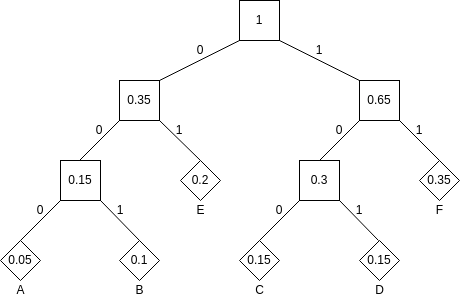
\includegraphics[scale=0.7]{huffman_tree.png}
    \caption{Huffman tree corresponding to the output code}
    \label{fig:huffman_tree}
    \end{figure}

\paragraph{}To generate a Huffman code of any (output) alphabet size, several changes would be necessary both in our data structure and in our algorithm:
\begin{itemize}
    \item Data structure
        \begin{itemize}
            \item We would need to add a field to store the alphabet size $N$ which was implicitly set to 2 in the binary Huffman code.
            \item We would need to store the $N$ children of each node which is not a leaf instead of the two children in the binary Huffman code.
        \end{itemize}
    \item Algorithm
        \begin{itemize}
            \item We would need to take the $N$ lowest probability and link them to create new nodes instead of the two nodes with the lowest probability in the binary Huffman code.
            \item We would need to assign a given unique symbol of the code to each child of a node when recursively building the Huffman code instead of 1 and 0 in the binary Huffman code where there were only 2 children per node.
            \item We might have to deal with problems of number of symbols and size of the alphabet not compatible unlike in the binary Huffman code where it is always possible to merge the two lowest probable nodes. 
        \end{itemize}
\end{itemize}

\subsection{On-line Lempel-Ziv algorithm (question 2)}

\paragraph{}The example given in the course about state of the art in data compression on slide 50/53 where the sequence 1011010100010 is encoded gives this output our \texttt{LZ\_online} function:
\begin{itemize}
    \item Dictionnary: \{'': (0, ''), '1': (1, '1'), '0': (2, '00'), '11': (3, '011'), '01': (4, '101'), '010': (5, '1000'), '00': (6, '0100'), '10': (7, '0010')\}
    \item Encoded sequence: 100011101100001000010
\end{itemize}

\subsection{Comparison between the two versions of the Lempel-Ziv algorithm (question 3)}
\paragraph{}The basic version has one main problem which is address coding. It needs to know the
size of the dictionary before an address encoding. The on-line version solves this problem by using the current dictionary size to determine the number of bits which is equal to $\lceil\log_2{N}\rceil$, where $N$ is the dictionary size. It is thus decreasing the size of the encoded text. This on-line variant is most of the time not very competitive in
terms of optimality but is very robust because it does not need assumptions about source behaviour and can thus allow an insteantaneous coding without having to browse the dictionary multiple times. The asympotic performances are reached only when the dictionary starts to become
representative: when it contains a significant fraction of sufficiently long typical messages.

\subsection{Implementation of the Lempel-Ziv 77 algorithm (question 4)}
\paragraph{}Running the example given in Figure 2 with our function and taking a \texttt{window\_size} of size 7 gives us this output: [(0, 0, 'a'), (0, 0, 'b'), (0, 0, 'r'), (3, 1, 'c'), (2, 1, 'd'), (7, 4, 'd')]. We have chosen to set the size of the look ahead buffer to the size of the window because it allows to have longer matches prefix and the prefix can not be longer than the this size.

%%%%%%%%%%%%%%%%%%%%%%%%%%%%%%%%%%%%%%%%%%

\end{document}